% !TeX root = ../thesis.tex

\chapter{Fundamentals and Related Work}
\label{sec:fundamentals_related-work}
\section{Overview}

The new era of deep neural networks began in 2012, when Krizhevsky et al. published
their results\cite{krizhevsky_imagenet_2017} on the ImageNet Large-scale Visual Recognition Challenge (ILSVRC)\cite{deng_imagenet_2009} . Their deep neural network (DNN) has 5 convolutional layers followed by 2 fully connected layers, which is approximately higher than the closest competitor based on SIFT\cite{sanchez_high-dimensional_2011}. The classification error rate is 10\%. For DNN, this moment is a huge breakthrough because they proved superior to classic computer vision methods. There are multiple factors that contribute to this achievement, such as
The training network can perform multiple orders of magnitude more powerful hardware than before and more training iterations, new training algorithms and network convolutional layer architectures.

Since then, many DNN methods for image classification and object detection have been developed. In the next section, we will review these methods. The existing methods can be divided into two groups: region proposal methods and end-to-end learning methods. The former includes regions proposal step and the proposed DNN classifier for proposed regions, the latter is a DNN, which is used to obtain the original image and directly output information about the detected object.
\subsection{Region Proposal Method}

Krizhevsky et al.\cite{krizhevsky_imagenet_2017} showed that DNN is a powerful tool for image classification. The conversion from the classification task to the detection network can be realized by classifying each possible sub-window of the image. However, this method requires huge computing power, because each image must run the classifier thousands times. The idea of region proposal solves this problem. It aims to suggest promising locations by using algorithms that are orders of magnitude faster than the classifier, thereby reducing the elevation window (number of runs of the classifier) for each image. Selective search\cite{uijlings_selective_2013} or edge boxes\cite{fleet_edge_2014} are examples of region proposal methods. 

R-CNN by Girshick et al.\cite{girshick_rich_2014} uses selective search. It is a three-stage object detector with a selective search region proposal generator, which is further processed by DNN (the same as that used by Krizhevsky et al.\cite{krizhevsky_imagenet_2017}) into 4096 feature vectors, which is then processed and classified by SVM. This method works well, but the speed is very slow, because each image on the Tesla K20 GPU takes 18 seconds.

He et al.\cite{he_spatial_2014} introduced the Spatial Pyramid Pool (SPPNet), in order to speeds up the calculation of R-CNN. It avoids re-evaluating the entire DNN on each proposal window by running the convolutional layer on the entire image and then pooling the feature maps, thereby creating a fixed-size grid (\(1\times1\), \(2\times2\), \(3\times3\), and \(6\times6\) ). Then, by concatenation the pooled vectors from the grid cells,a fixed-size feature vector (4096 elements) is created for each object. 

SPPNet inspired the authors of R-CNN to create the Fast R-CNN\cite{ren_faster_2016} version of their algorithm. It speeds up the calculation in the same way as in SPPNet, but only uses one pyramid layer (\(7\times7\). Similarly, the SVM on the output is replaced by fully connected layers. These layers predict the probability of the class. Interestingly, they also directly bound the coordinates of the box.

At the same time, Simonyan et al. are experimenting with very deep convolutional networks\cite{simonyan_very_2015}, in which they only use 3 to 3 convolutions and created a very successful VGGNet, which has up to 19 layers and is used in many subsequent papers, for example,\cite{ren_faster_2016,chen_3d_nodate}.

Ren et al. is one of them. They introduced Faster R-CNN\cite{ren_faster_2016} using the VGG-16 network architecture. Most importantly, they replace selective search with a region proposal network (RPN), which shares a convolutional layer with a classification DNN. RPN is basically a sliding window on a feature map, and each window position outputs an objectivity score and 9 bounding boxes (for 9 anchor boxes-3 ratios, 3 aspect ratios). Then, these proposals are classified in Fast R-CNN. The algorithm can reach about 15fps, and the performance is very good. 

He et al. even further improved the Faster R-CNN framework\cite{he_deep_2015} and their ResNet. It adds the remaining connections-shortcuts to the network, which makes the network only understand the difference between the input and output of the building blocks. This allows the use of SGD to train very deep networks because their design will not be affected much by gradient decay. Although the depth is very deep, the network is not as complicated as VGG-16\cite{simonyan_very_2015}. This is one of the newest and most advanced networks on ImageNet.
\paragraph{3D Bounding Box Detection for Autonomous Driving Applications}

\subsection{End-to-end Systems}

Sermanet et al. used another method in OverFeat\cite{sermanet_overfeat_2014}. They used a Fully Convolutional Network (FCN) to predict the object of each grid unit of width/12\(\times\)height/12 grid, and then fused the prediction to get the output position, thus avoiding the use of object suggestion generators. This method has been shown to be faster than R-CNN, but worse \cite{girshick_rich_2014}. 
\section{Datasets}
\begin{enumerate}
\item\textit{KITTI}


The whole work is mainly based on PointPillars\cite{lang_pointpillars_2019}. It has fast inference speed and relative higher detection accuracy.

For adversarial attack the work is based on KITTI\cite{geiger_vision_2013} dataset. This dataset is proposed relative earlier and famous in autonomous driving field. But it didn't consider adverse weather problem.

For adverse weather simulation, the work is based on DENSE\cite{heinzler_cnn-based_2020} dataset. This work have shown how to use this dataset to segment points with weather class. This dataset have collected the point cloud in chamber with man-made adverse weather, there's also clean point cloud. 

\end{enumerate}
CNN
Convolution
PointNet
Adversarial attacks
\begin{figure}[!htbp]
    \centering
    \subfigure[Logo 1]{
        
\includegraphics[width = \textwidth / 2 ]{Logos/KITLogo_RGB.pdf}
        \label{fig:logo1}
    }
    \hspace{10pt}
     %add desired spacing between images, e. g. ~, \quad, \qquad, \hfill etc.
     %(or a blank line to force the subfigure onto a new line)
    \subfigure[Logo 2]{
        
\includegraphics[width = \textwidth / 2 ]{Logos/KITLogo_RGB.pdf}
        \label{fig:logo2}
    }
    \caption[Short Description for List of Figures]{Long Description for under the figure.}
    \label{fig:logo1and2}
\end{figure}

\section{Evaluation of Adversarial Attacks}
\begin{enumerate}
\item\textit{Intersection over union}

Intersection over union means the similarity of two bounding boxes. It is used to compare detected bounding boxes and ground truth bounding boxes. 2D version is shown here:
\begin{center}
          \(IOU_{b_{1},b_{2}} = \frac{A(b_{1}\cap b_{2})}{A(b_{1}\cup b_{2})} \)
\end{center}
where \(A(\bullet)\) represents Area and b, are bounding boxes. For KITTI\cite{geiger_vision_2013} evaluation there's two criterions, \(IOU\geq0.5\) and \(IOU\geq0.7\) to accept a detection as a correct one.

\item\textit(Average Precision)
Precision is the ratio of detected objects \(TP+FP\), which are detected correctly. It shows how many false positive \(FP\) detections the detectors produces. It is defined as follows
\begin{center}
          \(Precision = \frac{TP}{TP+FP} \)
\end{center}
Recall represents the ratio of the ground truth objects \(TP+FN\), which are detected by the detector. It is defined as 
\begin{center}
          \(Recall = \frac{TP}{TP+FN} \)
\end{center}
Average precision (AP) is used in the KITTI benchmark. It samples the precision/recall curve on 11 places, interpolates it and computes the arithmetic mean. Therefore, this measure gives insight into how the precision/recall curve changes. For details see\cite{everingham_pascal_2010}

\end{enumerate}

\section{FGSM and Its Variants}

\begin{enumerate}
\item \textit{FGSM}

FGSM is shorten for fast gradient sign method\cite{goodfellow_explaining_2015}. It uses sign function with gradients, which get from loss function. As the panda example (Figure 4.1) shows the process of FGSM. The left picture is clean image, the classifier predicts the picture a panda. When perturbation is added to the clean image, even the epsilon value is very small, classification result is totally different, the panda is recognized as a gibbon.
\begin{center}
          \(x_{adv} = x + \epsilon sign(\nabla_{x}J(f(x;\theta),y) \)
\end{center}
\begin{figure}[!htbp]
\centering
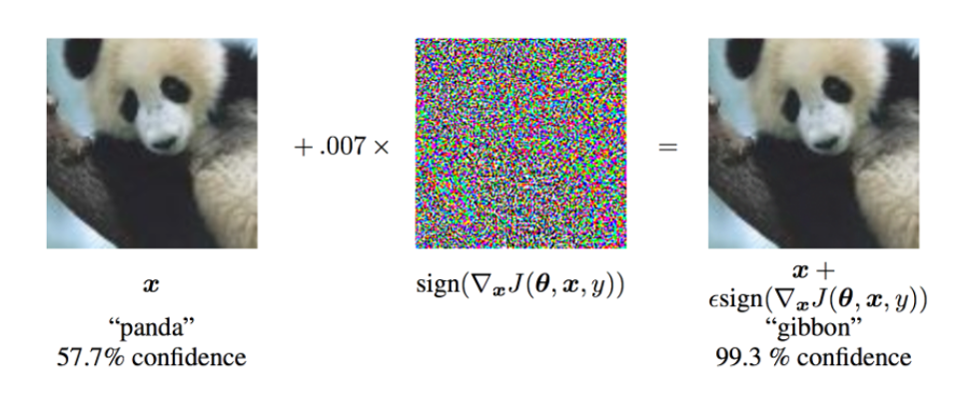
\includegraphics[scale=0.5]{FGSM.png}
\caption{Adversarial attack process of FGSM example}
\label{fig:FGSM}
\end{figure}
\item \textit{IFGSM} 

IFGSM\cite{kurakin_adversarial_2017} is shorten for iterative fast gradient sign method. This method improves FGSM and is also proposed by Goodfellow and his partners. IFGSM applies FGSM multiple times with a small step size. IFGSM performs better than FGSM. When the same clean image is attacked by FGSM and IFGSM with the same total epsilon, the impact of FGSM attack can be easily observed by naked eyes, but attack in IFGSM is imperceptible.
\begin{center}
          \(X_{0}^{adv} = X,  X_{N+1}^{adv}=Clip_{X,\epsilon}{X_{N}^{adv}+\alpha sign(\nabla_{x}J(f(X_{N}^{adv};\theta),y_{true}))} \)
\end{center}
 \item \textit{MIFGSM}
 
 MIFGSM\cite{dong_boosting_2018} is shorten for iterative fast gradient sign method with momentum. This method stabilizes optimization by accumulating gradients at each iteration.
  \begin{center}
          \(x^{*}_{t+1} =x^{*}_{t}+\alpha \frac{g_{t+1}}{\|g_{t+1}\|_{2}},
           g_{t+1} = \mu * g_{t}+\frac{J(X^{*}_{t},y^{*})}{\|\nabla_{x}J(X_{t}^{*},y^{*}\|_{1}} \)
\end{center}
 \item \textit{PGD}
 
 PGD\cite{madry_towards_2019} is shorten for projected gradient descent. Compared with IFGSM, this approach adds random initialization perturbation at the beginning.
 \begin{center}
          \(x^{t+1} =\prod_{x+S}({x^{T}+\alpha sign(\nabla_{x}L(\theta;x;y)))} \)
\end{center}
 
 \item \textit{Fast Gradient Norms}
 
 S in FGSM is sign, which represents  \(L_\infty\) norm. DeepFool\cite{moosavi-dezfooli_deepfool_2016} proposed  \(L_2\) norm to replace sign norm for a better result in image. 
 \begin{center}
          \(x^{*} =x+\sigma\frac{\nabla_{x}J(x,y)}{\|\nabla_{x}J(x,y)\|_{2}} \)
\end{center}
 There's also  \(L_1\) norm as Manhattan metric to replace sign norm. Liu et.al(\cite{liu_adversarial_2019}) proposed a new version of \(L_2\) norm named \(L_2.5\) norm, which is normalized \(L_2\) norm's result. 
 \item \textit{Attack on Different Features} 
 
 LiDAR point clouds have 4 dimensions which are 4 features: \(x\) coordinate, \(y\) coordinate, \(z\) coordinate and intensity \(r\). So there are two different kinds of attack types: one is only attack one feature, which is separately attack \(x\) coordinate, \(y\) coordinate, \(z\) coordinate and intensity \(r\). The other is attack multiple features: \(xyz\) coordinates, and the combination of \(xyz\) coordinates and intensity \(r\). 

\item\textit{Adversarial training}

FGSM-based Adversarial training is an efficient way to defense adversarial attacks of FGSM. The adversarial training of FGSM:
\begin{center}
          \(Loss_{train} = 1/2*(Loss_{original}+Loss_{perturbation}) \)
\end{center}

\end{enumerate}
